In this strategy, an initial solution is obtained on an initial mesh with a set of canonical refinement zones that are usually used for a flow over an airfoil. We refer to this mesh as M0\_nz25, see Figure \ref{fig:M0_mesh}. In-plane mesh sizes are indicated in the figure. The initial mesh spacing/resolution on the surface of the airfoil in the streamwise and spanwise directions is set to be below 75 and 40 in wall units, respectively.
Here nz25 refers to the number of spanwise extruded layers (i.e., 25) used in this mesh. 
As mentioned before, the VMS-based error estimator is applied to phase-averaged data, and the maximum error value over multiple phases (i.e., at 24 equispaced phases over the surging cycle), and over the spanwise direction, is selected to represent the element-level local error within the airfoil plane/section throughout the surging cycle. 
The element-level error estimated on this mesh is shown in Figure \ref{fig:M0_err_plot}. 
We can see that higher errors are observed primarily in the regions traversed by the LEV through the surging cycle, as well as in the wake of the airfoil. 
Higher errors are also observed close to the airfoil surface and in the boundary layer region.

Based on the estimated error, the mesh is refined by a factor of 2 in zones where high error values are found, including in the boundary layer mesh (i.e., along the streamwise direction). 
The spanwise resolution is also refined by a factor of 2 (i.e., the number of layers in the spanwise direction is doubled). 
This adapted mesh is shown in Figure \ref{fig:Mza1_mesh} and the estimated error on it is shown in Figure \ref{fig:Mza1_err_plot}. It is referred to as the Mza1\_nz50 mesh (where za is short for zonal adaptation and 1 in za1 denotes the first iteration of mesh adaptation).
%It is observed that the error has approximately reduced by a factor of 4 in the Mza1\_nz50 mesh as compared to the M0 mesh.
It is observed that the error has reduced in the Mza1\_nz50 mesh as compared to the M0 mesh
These meshes, M0\_nz25 and Mza1\_nz50, consist of 774,525 and 2,874,300 elements, respectively.

%Zonal refinements are added to the Mza1 mesh in regions of high error, and the mesh is refined further by a factor of 2 in these zones, along with the boundary layer mesh in the streamwise direction, and the number of layers in the spanwise direction is doubled.  This mesh, which is referred to as Mza2, is shown in Figure \ref{fig:Mza2_mesh}. Again, we observe that the error has reduced by a factor of 4 in the Mz\_a2 mesh as compared to Mz\_a1 mesh.

%The number of elements for each mesh is presented in Table \ref{table:mesh_zonal_summary}.


% \begin{table}[H]
% 	\centering
% 	\caption{Summary of zonal refinement based meshes}
% 	\label{table:mesh_zonal_summary}
% 	\begin{tabular}{|l|c|c|c|c|c|}
% 		\hline
% 		Mesh case  & No. of elements\\
% 		\hline
% 		\hline
% 		M0\_nz25 & 774,525 \\
% 		\hline
% 		Mza1\_nz50 &  2,874,300 \\
% 		\hline
% %		Mz\_a2 & 14,329,200 \\
% %		\hline
% 	\end{tabular}
	
% \end{table}

A comparison of different adaptive strategies/adapted meshes is provided in Section \ref{sec:results_adapt}.

\begin{figure}[H]
\centering
\begin{subfigure}[b]{0.475\textwidth}
\centering
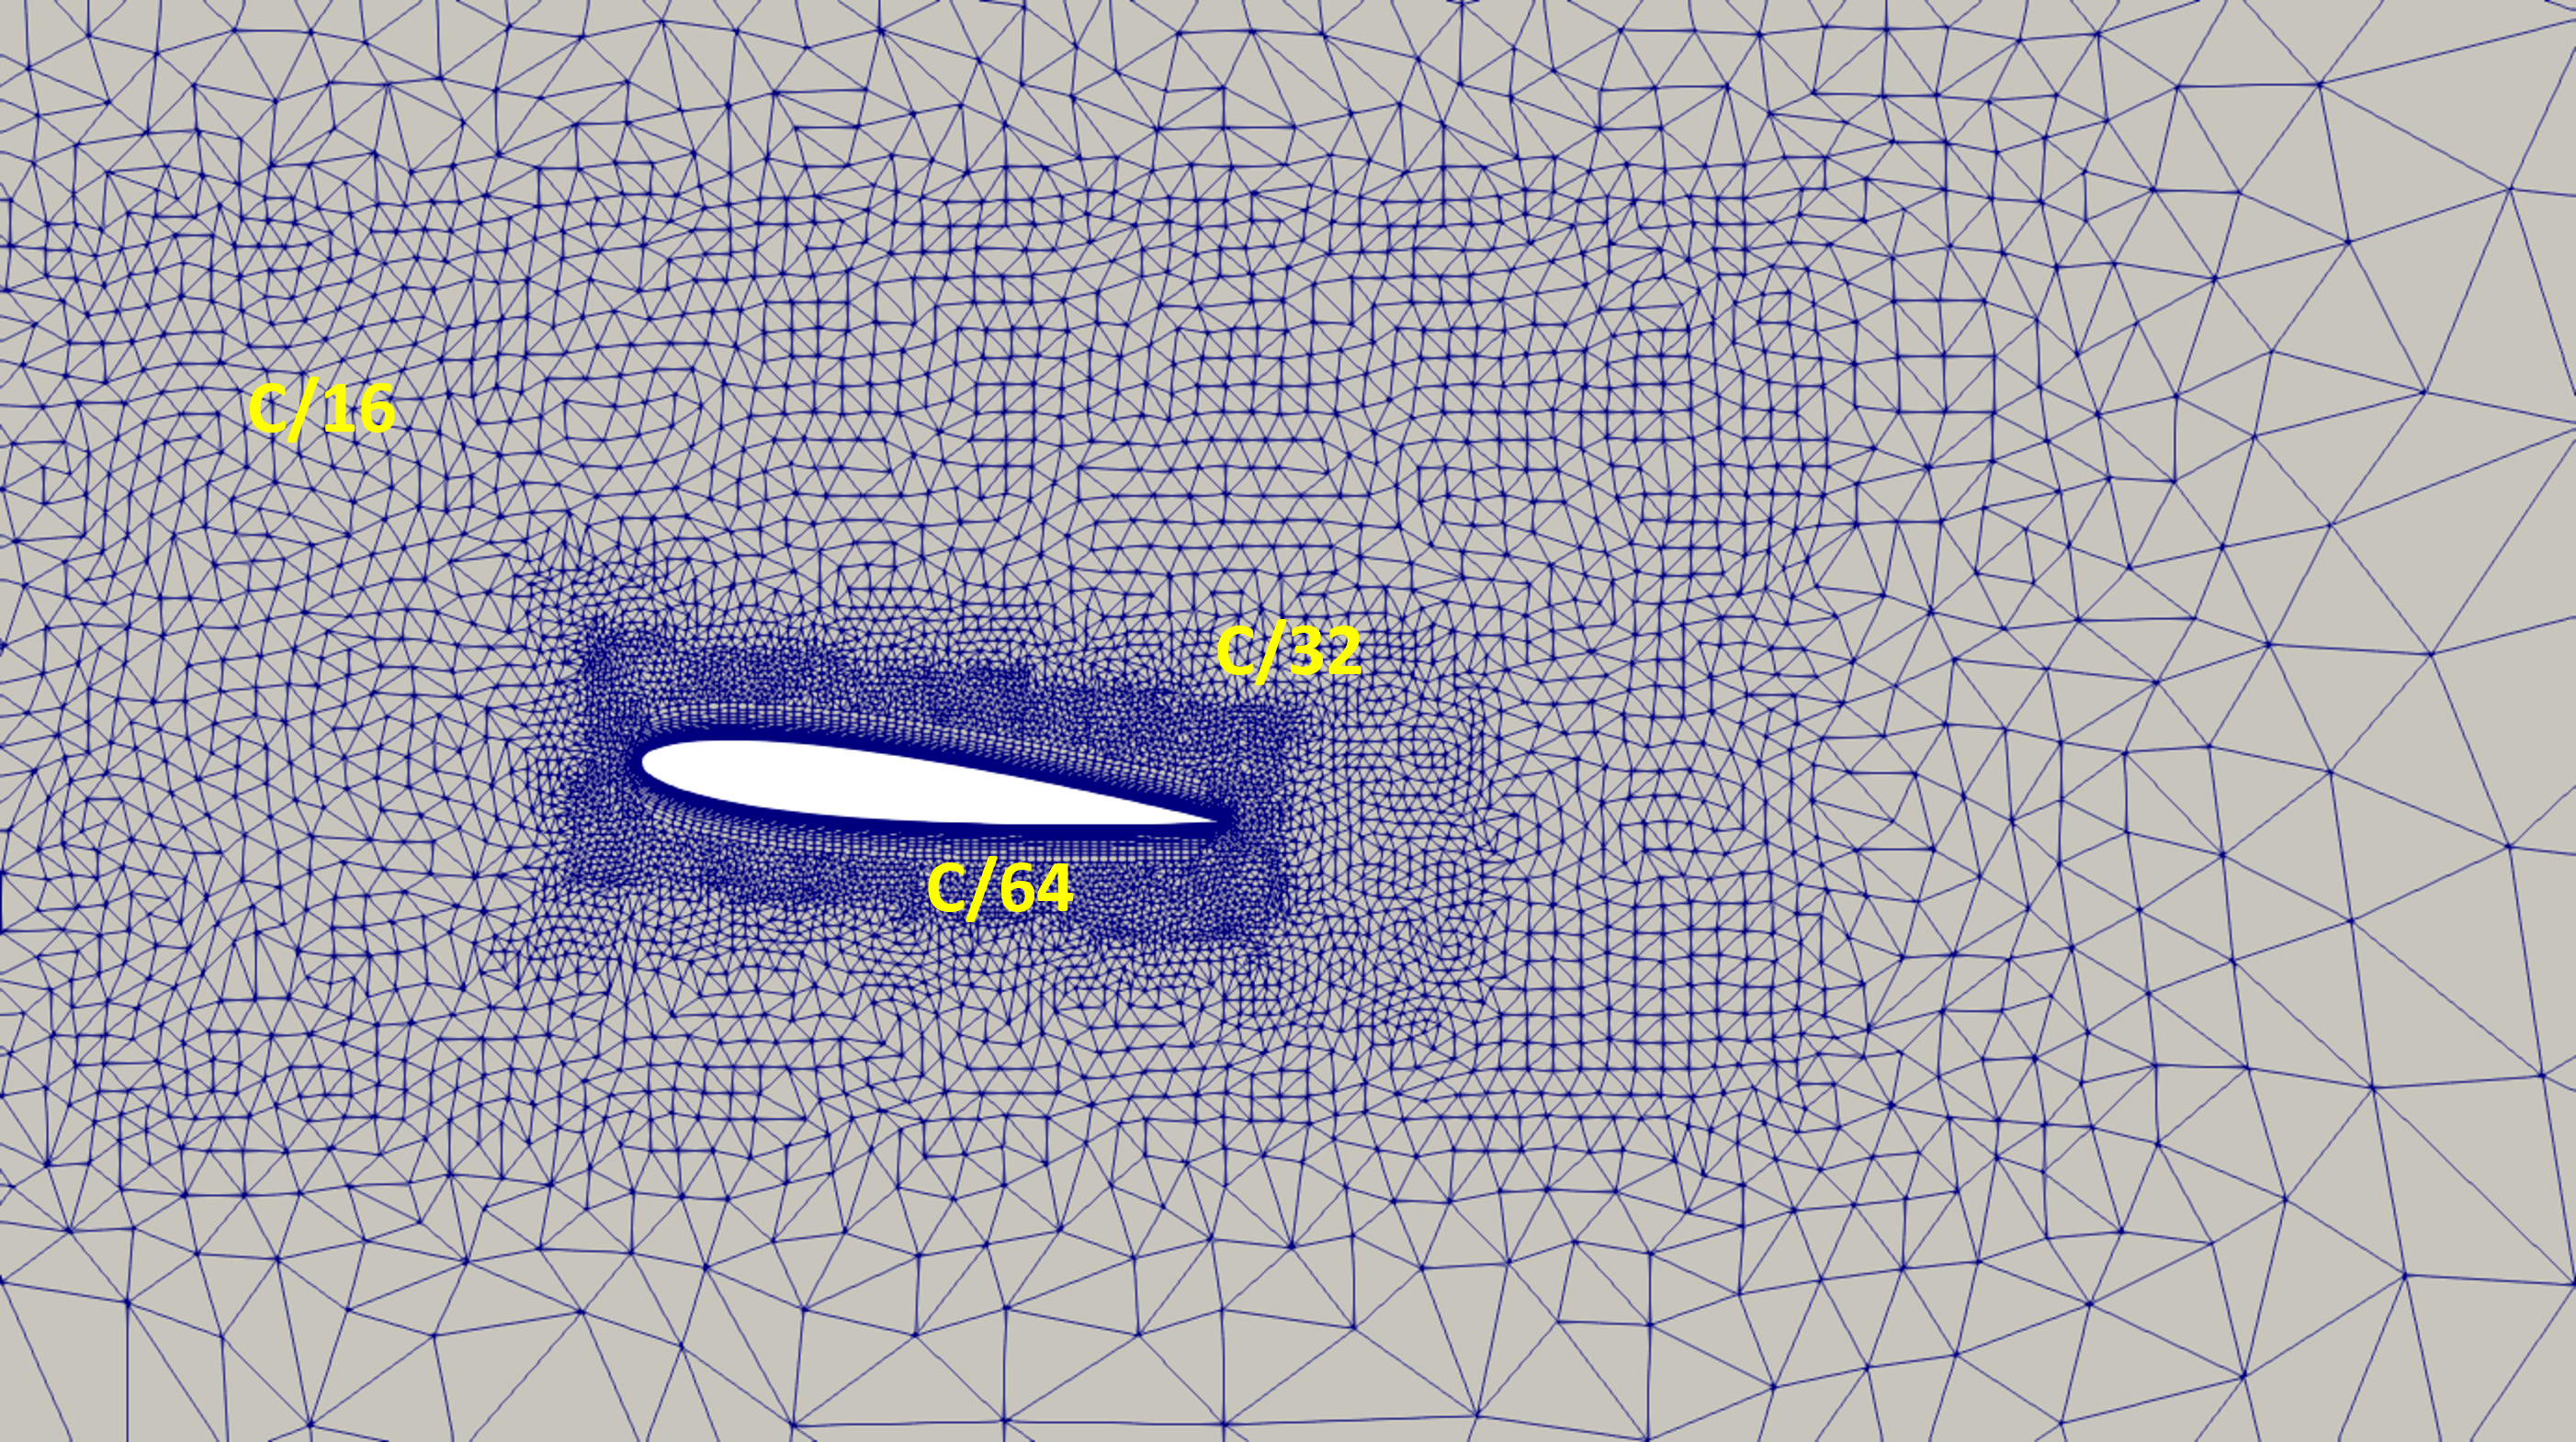
\includegraphics[width=1\textwidth]{figures/adapt_strat/M0_mesh.png}
\caption{M0\_nz25 mesh}
\label{fig:M0_mesh}
\end{subfigure}
\begin{subfigure}[b]{0.475\textwidth}
\centering
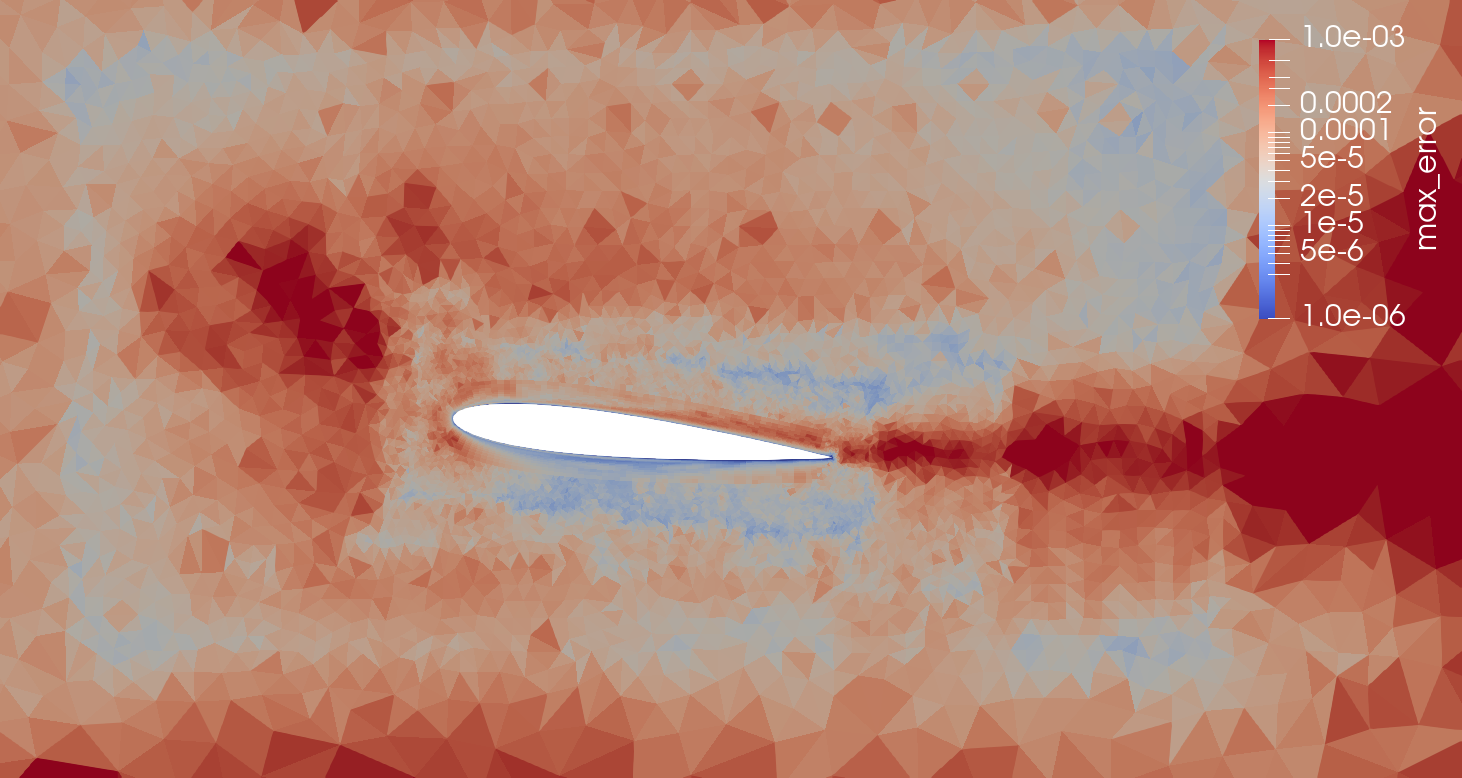
\includegraphics[width=1\textwidth]{figures/adapt_strat/M0_error.png}
\caption{M0\_nz25 error field}
\label{fig:M0_err_plot}
\end{subfigure}
\begin{subfigure}[b]{0.475\textwidth}
\centering
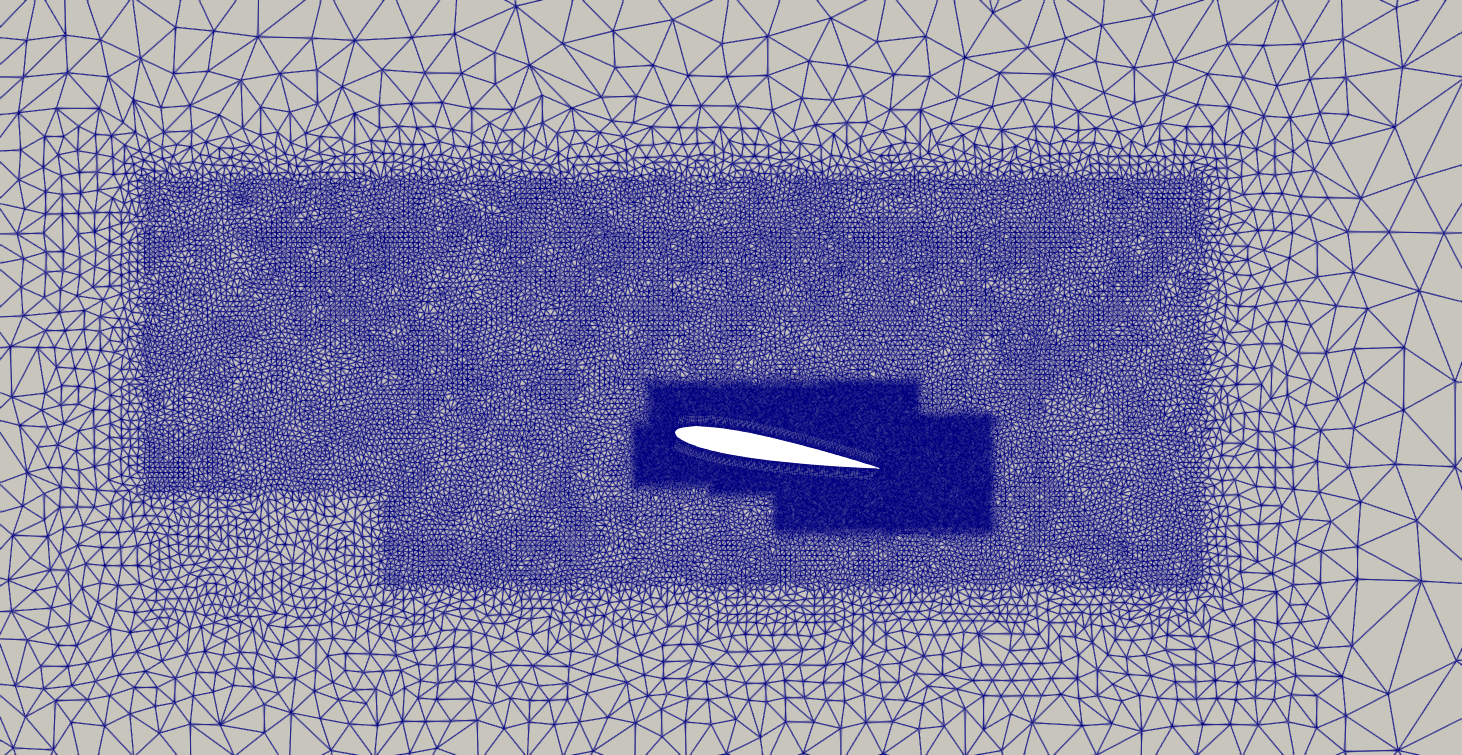
\includegraphics[width=1\textwidth]{figures/adapt_strat/Mza1_mesh.png}
\caption{Mza1\_nz50 mesh}
\label{fig:Mza1_mesh}
\end{subfigure}
\begin{subfigure}[b]{0.475\textwidth}
\centering
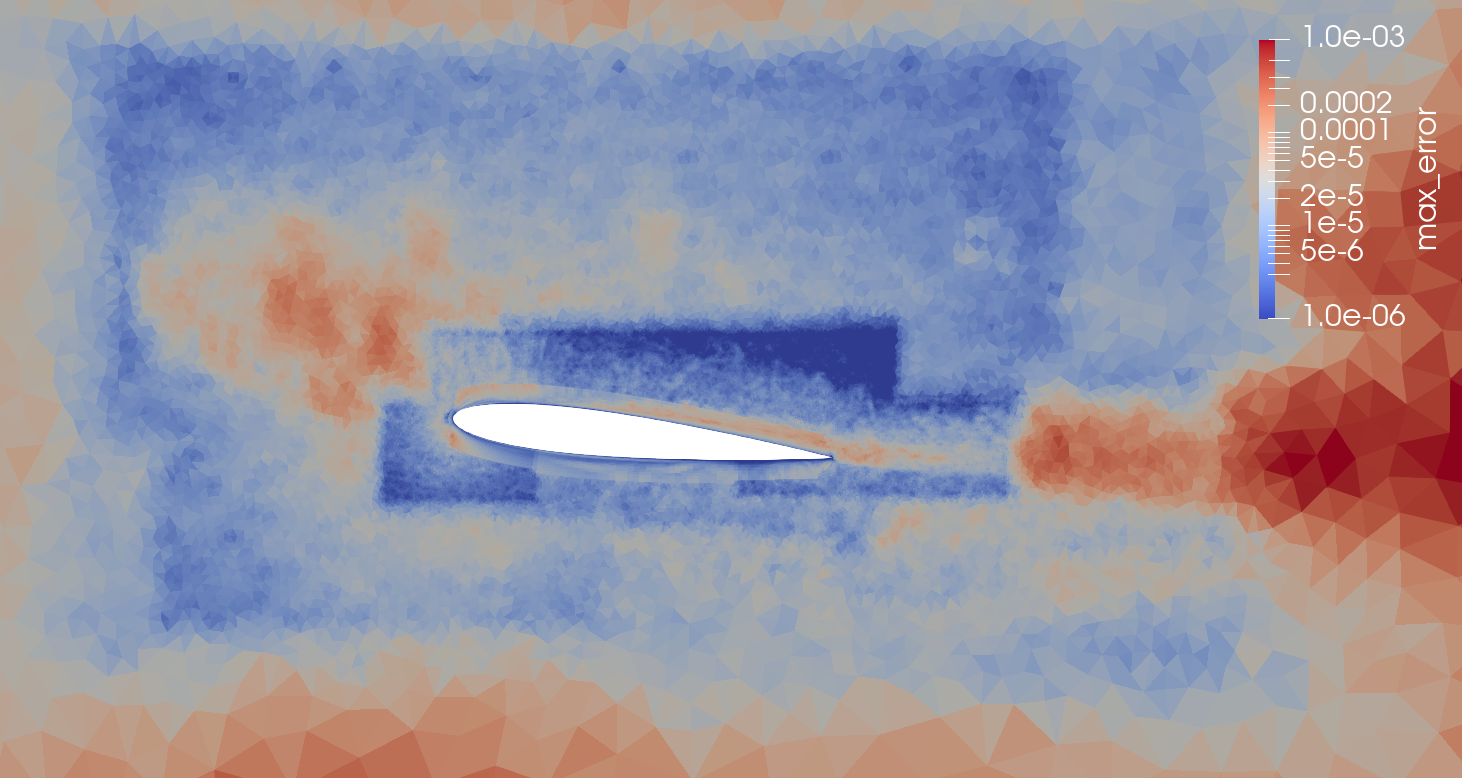
\includegraphics[width=1\textwidth]{figures/adapt_strat/Mza1_error.png}
\caption{Mza1\_nz50 error field}
\label{fig:Mza1_err_plot}
\end{subfigure}
%\begin{subfigure}[b]{0.475\textwidth}
%\centering
%\includegraphics[width=1\textwidth]{figures/adapt_strat/Mza2_mesh.png}
%\caption{Mz\_a2 mesh}
%\label{fig:Mza2_mesh}
%\end{subfigure}
%\begin{subfigure}[b]{0.475\textwidth}
%\centering
%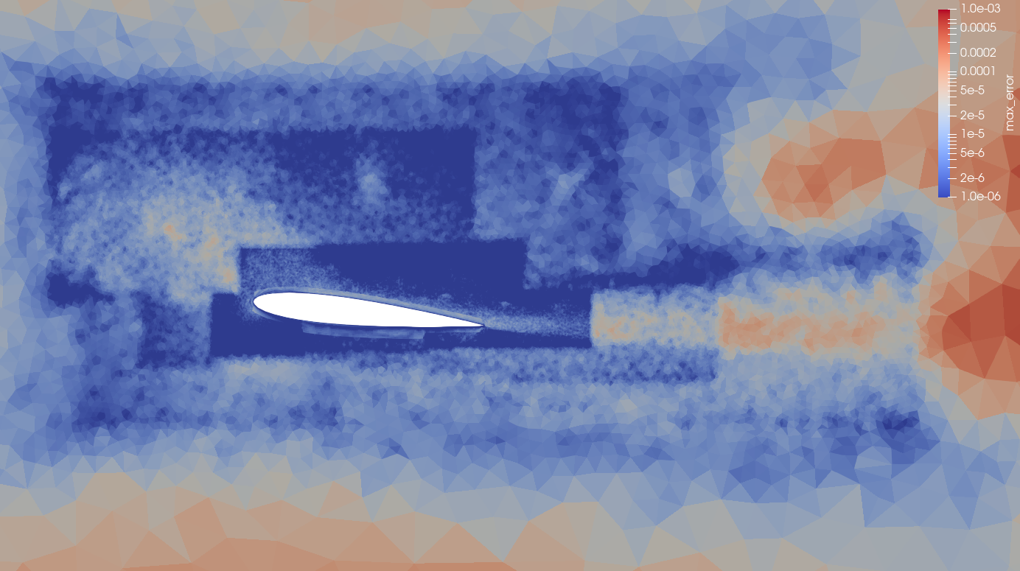
\includegraphics[width=1\textwidth]{figures/adapt_strat/Mza2_error_plot.png}
%\caption{Mz\_a2 error field}
%\label{fig:Mza2_err_plot}
%\end{subfigure}
\caption{Meshes and estimated error fields for zonal-based strategy}
\end{figure}

